% Options for packages loaded elsewhere
\PassOptionsToPackage{unicode}{hyperref}
\PassOptionsToPackage{hyphens}{url}
%
\documentclass[
  man]{apa6}
\usepackage{amsmath,amssymb}
\usepackage{lmodern}
\usepackage{iftex}
\ifPDFTeX
  \usepackage[T1]{fontenc}
  \usepackage[utf8]{inputenc}
  \usepackage{textcomp} % provide euro and other symbols
\else % if luatex or xetex
  \usepackage{unicode-math}
  \defaultfontfeatures{Scale=MatchLowercase}
  \defaultfontfeatures[\rmfamily]{Ligatures=TeX,Scale=1}
\fi
% Use upquote if available, for straight quotes in verbatim environments
\IfFileExists{upquote.sty}{\usepackage{upquote}}{}
\IfFileExists{microtype.sty}{% use microtype if available
  \usepackage[]{microtype}
  \UseMicrotypeSet[protrusion]{basicmath} % disable protrusion for tt fonts
}{}
\makeatletter
\@ifundefined{KOMAClassName}{% if non-KOMA class
  \IfFileExists{parskip.sty}{%
    \usepackage{parskip}
  }{% else
    \setlength{\parindent}{0pt}
    \setlength{\parskip}{6pt plus 2pt minus 1pt}}
}{% if KOMA class
  \KOMAoptions{parskip=half}}
\makeatother
\usepackage{xcolor}
\IfFileExists{xurl.sty}{\usepackage{xurl}}{} % add URL line breaks if available
\IfFileExists{bookmark.sty}{\usepackage{bookmark}}{\usepackage{hyperref}}
\hypersetup{
  pdftitle={Item Characteristic Curve specification from Classical Test Theory Indices},
  pdfauthor={Diego Figueiras1 \& John T. Kulas1},
  pdflang={en-EN},
  pdfkeywords={keywords},
  hidelinks,
  pdfcreator={LaTeX via pandoc}}
\urlstyle{same} % disable monospaced font for URLs
\usepackage{graphicx}
\makeatletter
\def\maxwidth{\ifdim\Gin@nat@width>\linewidth\linewidth\else\Gin@nat@width\fi}
\def\maxheight{\ifdim\Gin@nat@height>\textheight\textheight\else\Gin@nat@height\fi}
\makeatother
% Scale images if necessary, so that they will not overflow the page
% margins by default, and it is still possible to overwrite the defaults
% using explicit options in \includegraphics[width, height, ...]{}
\setkeys{Gin}{width=\maxwidth,height=\maxheight,keepaspectratio}
% Set default figure placement to htbp
\makeatletter
\def\fps@figure{htbp}
\makeatother
\setlength{\emergencystretch}{3em} % prevent overfull lines
\providecommand{\tightlist}{%
  \setlength{\itemsep}{0pt}\setlength{\parskip}{0pt}}
\setcounter{secnumdepth}{-\maxdimen} % remove section numbering
% Make \paragraph and \subparagraph free-standing
\ifx\paragraph\undefined\else
  \let\oldparagraph\paragraph
  \renewcommand{\paragraph}[1]{\oldparagraph{#1}\mbox{}}
\fi
\ifx\subparagraph\undefined\else
  \let\oldsubparagraph\subparagraph
  \renewcommand{\subparagraph}[1]{\oldsubparagraph{#1}\mbox{}}
\fi
\newlength{\cslhangindent}
\setlength{\cslhangindent}{1.5em}
\newlength{\csllabelwidth}
\setlength{\csllabelwidth}{3em}
\newlength{\cslentryspacingunit} % times entry-spacing
\setlength{\cslentryspacingunit}{\parskip}
\newenvironment{CSLReferences}[2] % #1 hanging-ident, #2 entry spacing
 {% don't indent paragraphs
  \setlength{\parindent}{0pt}
  % turn on hanging indent if param 1 is 1
  \ifodd #1
  \let\oldpar\par
  \def\par{\hangindent=\cslhangindent\oldpar}
  \fi
  % set entry spacing
  \setlength{\parskip}{#2\cslentryspacingunit}
 }%
 {}
\usepackage{calc}
\newcommand{\CSLBlock}[1]{#1\hfill\break}
\newcommand{\CSLLeftMargin}[1]{\parbox[t]{\csllabelwidth}{#1}}
\newcommand{\CSLRightInline}[1]{\parbox[t]{\linewidth - \csllabelwidth}{#1}\break}
\newcommand{\CSLIndent}[1]{\hspace{\cslhangindent}#1}
\ifLuaTeX
\usepackage[bidi=basic]{babel}
\else
\usepackage[bidi=default]{babel}
\fi
\babelprovide[main,import]{english}
% get rid of language-specific shorthands (see #6817):
\let\LanguageShortHands\languageshorthands
\def\languageshorthands#1{}
% Manuscript styling
\usepackage{upgreek}
\captionsetup{font=singlespacing,justification=justified}

% Table formatting
\usepackage{longtable}
\usepackage{lscape}
% \usepackage[counterclockwise]{rotating}   % Landscape page setup for large tables
\usepackage{multirow}		% Table styling
\usepackage{tabularx}		% Control Column width
\usepackage[flushleft]{threeparttable}	% Allows for three part tables with a specified notes section
\usepackage{threeparttablex}            % Lets threeparttable work with longtable

% Create new environments so endfloat can handle them
% \newenvironment{ltable}
%   {\begin{landscape}\centering\begin{threeparttable}}
%   {\end{threeparttable}\end{landscape}}
\newenvironment{lltable}{\begin{landscape}\centering\begin{ThreePartTable}}{\end{ThreePartTable}\end{landscape}}

% Enables adjusting longtable caption width to table width
% Solution found at http://golatex.de/longtable-mit-caption-so-breit-wie-die-tabelle-t15767.html
\makeatletter
\newcommand\LastLTentrywidth{1em}
\newlength\longtablewidth
\setlength{\longtablewidth}{1in}
\newcommand{\getlongtablewidth}{\begingroup \ifcsname LT@\roman{LT@tables}\endcsname \global\longtablewidth=0pt \renewcommand{\LT@entry}[2]{\global\advance\longtablewidth by ##2\relax\gdef\LastLTentrywidth{##2}}\@nameuse{LT@\roman{LT@tables}} \fi \endgroup}

% \setlength{\parindent}{0.5in}
% \setlength{\parskip}{0pt plus 0pt minus 0pt}

% Overwrite redefinition of paragraph and subparagraph by the default LaTeX template
% See https://github.com/crsh/papaja/issues/292
\makeatletter
\renewcommand{\paragraph}{\@startsection{paragraph}{4}{\parindent}%
  {0\baselineskip \@plus 0.2ex \@minus 0.2ex}%
  {-1em}%
  {\normalfont\normalsize\bfseries\itshape\typesectitle}}

\renewcommand{\subparagraph}[1]{\@startsection{subparagraph}{5}{1em}%
  {0\baselineskip \@plus 0.2ex \@minus 0.2ex}%
  {-\z@\relax}%
  {\normalfont\normalsize\itshape\hspace{\parindent}{#1}\textit{\addperi}}{\relax}}
\makeatother

% \usepackage{etoolbox}
\makeatletter
\patchcmd{\HyOrg@maketitle}
  {\section{\normalfont\normalsize\abstractname}}
  {\section*{\normalfont\normalsize\abstractname}}
  {}{\typeout{Failed to patch abstract.}}
\patchcmd{\HyOrg@maketitle}
  {\section{\protect\normalfont{\@title}}}
  {\section*{\protect\normalfont{\@title}}}
  {}{\typeout{Failed to patch title.}}
\makeatother

\usepackage{xpatch}
\makeatletter
\xapptocmd\appendix
  {\xapptocmd\section
    {\addcontentsline{toc}{section}{\appendixname\ifoneappendix\else~\theappendix\fi\\: #1}}
    {}{\InnerPatchFailed}%
  }
{}{\PatchFailed}
\keywords{keywords\newline\indent Word count: X}
\DeclareDelayedFloatFlavor{ThreePartTable}{table}
\DeclareDelayedFloatFlavor{lltable}{table}
\DeclareDelayedFloatFlavor*{longtable}{table}
\makeatletter
\renewcommand{\efloat@iwrite}[1]{\immediate\expandafter\protected@write\csname efloat@post#1\endcsname{}}
\makeatother
\usepackage{csquotes}
\ifLuaTeX
  \usepackage{selnolig}  % disable illegal ligatures
\fi

\title{Item Characteristic Curve specification from Classical Test Theory Indices}
\author{Diego Figueiras\textsuperscript{1} \& John T. Kulas\textsuperscript{1}}
\date{}


\shorttitle{CTT ICCs}

\authornote{

The authors made the following contributions. John T. Kulas: .

Correspondence concerning this article should be addressed to Diego Figueiras, Dickson Hall 226. E-mail: \href{mailto:figueirasd1@montclair.edu}{\nolinkurl{figueirasd1@montclair.edu}}

}

\affiliation{\vspace{0.5cm}\textsuperscript{1} Montclair State University}

\abstract{%
Item characteristic curves (ICC's) provide visual indication of important attributes of assessment items - most typically \emph{difficulty} and \emph{discrimination}. Assessment specialists who examine ICC's usually do so from within the psychometric framework of either Item Response Theory (IRT) or Rasch modeling. We propose an extension of this tradition of item characteristic visualization within the Classical Test Theory (CTT) framework. We first simulate binary (e.g., true \emph{test}) data with controlled item difficulty characteristics to generate linking parameters between the IRT and CTT difficulty indices. The results of these simulations provided some degree of confidence regarding functional linking invariance. Next, we simulated datasets of varying item characteristic specification and generated ICCs derived from both IRT and CTT frameworks. Differential item functioning (DIF) was implicated by calculating the geometric area between the IRT- and CTT- specified ogives. The DIF was \ldots. , providing a moderate degree of confidence regarding ICC comparability, providing assessment specialists with a visual tool regarding CTT-derived item characteristics. An \texttt{R} package, \texttt{ctticc}, performs the ICC estimations presented in the current paper.
}



\begin{document}
\maketitle

\begin{figure}
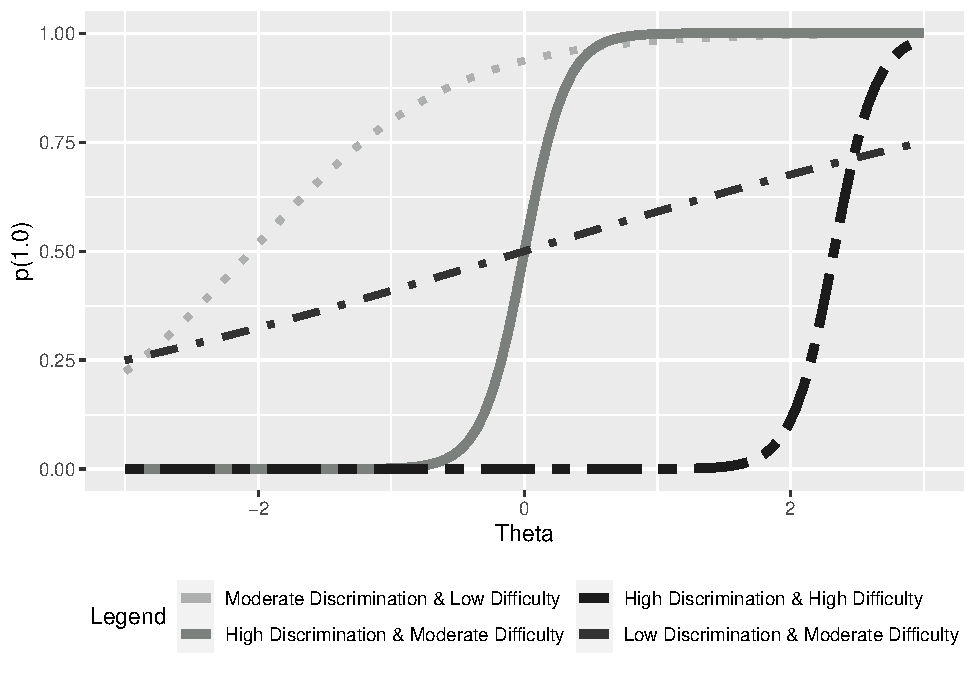
\includegraphics[width=1\linewidth,height=0.8\textheight]{ICC_project_files/figure-latex/example-1} \caption{Item characteristic curves reflecting predominant visual differences in difficulty and discrimination.}\label{fig:example}
\end{figure}

Item characteristic curves are frequently referenced by psychometricians as visual indicators of important attributes of assessment items - most commonly \emph{difficulty} and \emph{discrimination}. Within these visual presentations the x-axis ranges along ``trait'' levels (by convention typically denoted with the greek \(\theta\)), whereas the y-axis displays probabilities of responding to the item within a given response category. In the context of true tests, the response categories are binary, and the y-axis probability refers to the likelihood of a ``correct'' response. From this visualization, the observer extracts the likelihood that respondents of any trait level would answer a focal item correctly. If the curve transitions from low to high likelihood at a location toward the lower end of the trait (e.g., ``left'' on the plotting surface), this indicates that it is relatively easy to answer the item correctly. Stated in the parlance of IRT or Rasch traditions, it does not take much \(\theta\) to have a high likelihood of answering correctly. On the contrary, if the growth in the curve occurs primarily at higher trait levels, this indicates that the item is relatively more difficult. Through the lens of IRT, if discrimination is modeled and the curve is sharp (e.g., strongly vertical), this indicates high discrimination; if it is flatter, that is an indication of poorer discrimination (see Figure \ref{fig:example}).

Assessment specialists who examine ICC's usually do so from within the psychometric framework of either Item Response Theory (IRT) or Rasch modeling. These frameworks provide the parameters necessary to plot the ogive functions. Rasch models only estimate difficulty, and assume that differences in discrimination represent flaws in measurement. The IRT 2 parameter logistic model (2PL), however, models both item difficulty as well as item discrimination. Item difficulty (the \emph{b}-parameter) is scaled as the trait level associated with a 50\% likelihood of correct response (e.g., it is scaled to \(\theta\)). Item discrimination (\emph{a}-parameter) is the degree to which an item differentiates across individuals who are characterized as being relatively lower or higher on the trait. From a Classical Test Theory (CTT) orientation, item difficulty is most commonly represented by the percent of individuals answering the item correctly (also referred to as a \emph{p-value}). Item discrimination can be conveyed via a few different CTT indices, but the most commonly calculated and consulted index is the corrected item total correlation.

Assessment specialists who consult these CTT parameters don't typically (to our knowledge!) attempt to represent them visually, as is common in IRT and Rasch applications. However, there is perhaps little opposition for them not to do so, as ICC's based on CTT parameters could provide snapshot psychometric information as valuable as those gained from IRT- or Rasch-derived ICC's. The largest obstacle to psychometricians deeming CTT-derived visuals to be of value is likely tied to the concept of invariance, which refers to IRT parameter independence across item and person estimates. However, this property is often overstated, as invariance is only attained with perfect model-data fit (which never occurs), and is also only true after being subjected to linear transformation (commonly across samples). Additionally, several comparative investigations have noted commonality between IRT and CTT difficulty and discrimination estimates as well as relative stability of CTT estimates when samples are large and/or judisciously constructed (Fan, 1998). Fan in fact summarizes that the IRT and CTT frameworks ``\ldots produce very similar item and person statistics'' (p.379). Hambleton and Jones (1993) concluded that ``no study provides enough empirical evidence on the extent of disparity between the two frameworks and the superiority of IRT over CTT despite the theoretical differences''.

\hypertarget{ctt-and-irt-comparability-investigations}{%
\subsection{CTT and IRT comparability investigations}\label{ctt-and-irt-comparability-investigations}}

Fan (1998) looked at the correlations between ability estimates and item difficulty in CTT and all three IRT models. These correlations were very high, generally between .80 and .90, showing a lot of overlap between the two methodologies. As for item discrimination, correlations were moderate to high, with only a few being very low.\footnote{\ldots and in fact, as is presented below, the relationship between the IRT and CTT discrimination indices is non-linear - the correlation is an inappropriate index to capture the magnitude of this relationship.}

Fan (1998) also investigated item invariance for all models. In theory, the major advantage of IRT models over CTT is that the latter has an interdependency between the item and person statistics, whereas IRT has no such dependency. For example, within CTT examinations, the average item difficulty is equivalent to the average person score - these indices are merely reflective of averages computed across rows or columns. What Fan (1998) found in his study, however, did not support the purported invariant advantage of IRT parameters over CTT indices. Both CTT item difficulty and discrimination degrees of invariance were highly correlated with those of IRT, indicating that they were highly comparable.

There has also been occasions in which the invariance parameter has been conceptualized as a graded continuum instead of a categorical population property (Hambleton et al., 1991; Rupp \& Zumbo, 2004). Estimates of IRT parameters across different calibration runs can be looked at for evidence of a possible lack of invariance. This doesn't happen with CTT item parameters, since they will always be sample-dependent. This dependency, however, is greatly influenced by the sampling strategy. Large scale data, truly random sampling, and large range items could give comparable CTT item and person statistics across testing populations and occasions (Kulas et al., 2017). Additionally, there are several empirical investigations that note high levels of ``invariance'' of CTT estimates, in some cases surpassing IRT item estimates in their capacity to have cross-sample stability (Fan, 1998; Macdonald \& Paunonen, 2002).

An adjustment to Lord (2012)'s formula giving the functional relationship between the ``non-invariant'' CTT and ``invariant'' IRT statistics becomes useful in comparing the two methodologies, despite the supposed lack of invariance from CTT. So even though here we acknowledge that invariance is a categorical IRT property, we still follow the functional modification proposed by Kulas et al. (2017), noting that having a large sample that is truly random and whose items are normally distributed and have a center at the moderate difficulty can help reduce threats to CTT ``invariance''.

\hypertarget{relationship-between-irt-and-ctt-indices}{%
\subsection{Relationship between IRT and CTT indices}\label{relationship-between-irt-and-ctt-indices}}

Lord (2012) described a function that approximates the relationship between the IRT \emph{a}-parameter and the CTT discrimination index of an item-test biserial correlation:

\[a_i\cong \frac{r_i}{\sqrt{1-r_i^2}}\]

This formula wasn't intended for practical purposes but rather was specified in an attempt to help assessment specialists who were more familiar with CTT procedures to better understand the relationship to the IRT discrimination parameter. In an effort to move from the conceptual to a practical application, Kulas et al. (2017) proposed a modification that minimized the average residual (either \(a_i\) or \(r_i\), where \(r_i\) is the \emph{corrected} item-total \emph{point-biserial} correlation).

The Kulas et al. (2017) investigations (both simulated and utilizing real-world test data) identified systematic predictive differences across items with differing item difficulty values, so their recommended formula included a specification for item difficulty (this formulaic specification is also retained in the current presentation):

\[\hat{a_i}\cong[(.51 + .02z_g + .3z_g^2)r]+[(.57 - .009z_g + .19z_g^2)\frac{e^r-e^{-r}}{e-e^r}]\]

Where \(g\) is the absolute deviation from 50\% responding an item correctly and 50\% responding incorrectly (e.g., a ``p-value'' of .5). \(z_g\) is the standard normal deviate associated with \(g\). This transformation of the standard p-value was recommended in order to scale this index along an interval-level metric more directly analogous to the IRT \emph{b}-parameter. Figure 2 visualizes the re-specifications of Lord's formula at p-values (difficulty) of .5, .3 (or .7), and .1 (or .9) and highlights the nonlinear nature of this relationship - especially noticeable at high(er) levels of discrimination.

\begin{figure}
\centering
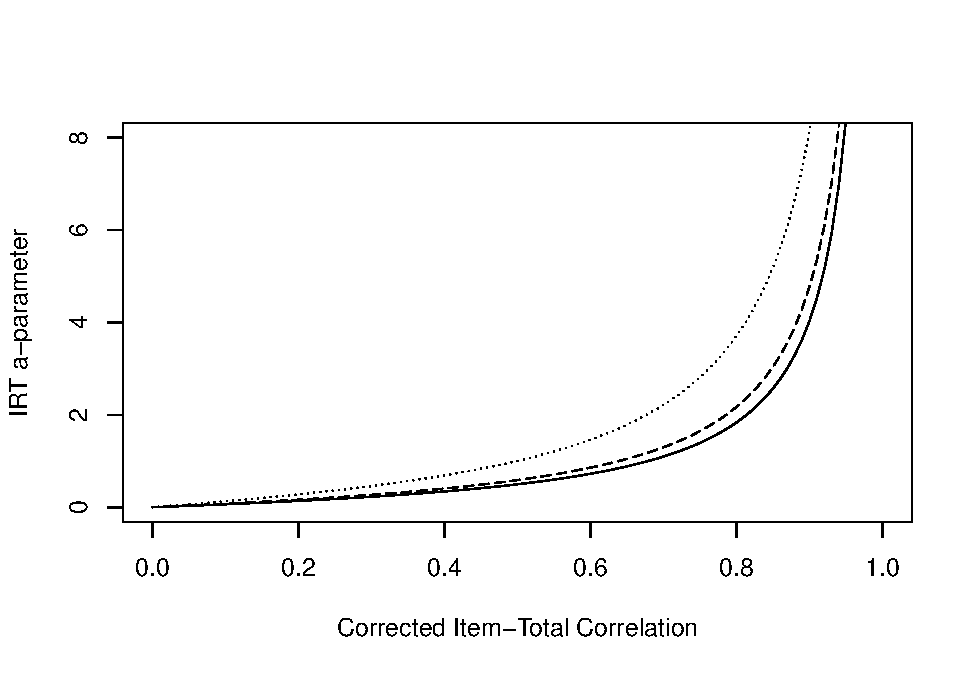
\includegraphics{ICC_project_files/figure-latex/acorrected-1.pdf}
\caption{\label{fig:acorrected}Empricially-derived functional relationship between the IRT \emph{a} parameter and the CTT corrected-item total correlation as a function of item difficulty (p-value; solid = .5, dashed = .3/.7, dotted = .1/.9).}
\end{figure}

As we can see, the higher the corrected item-total correlations, the higher the estimated IRT a-parameter (discrimination). Also, as the p-values (difficulty) deviates from 0, the relationship between the estimated IRT a-parameter and the corrected item-total correlations becomes stronger.

Practitioners and researchers that don't use IRT or Rasch models and instead opt to follow a CTT philosophy would benefit from having ICC's that use CTT statistics. This study intends to show evidence of the overlapping nature of CTT and IRT parameters when it comes to plotting ICCs.

\hypertarget{study-1a---establishing-relationship-between-the-irt-and-ctt-difficulty-indices.}{%
\section{Study 1A - Establishing relationship between the IRT and CTT difficulty indices.}\label{study-1a---establishing-relationship-between-the-irt-and-ctt-difficulty-indices.}}

\hypertarget{method}{%
\subsection{Method}\label{method}}

Although the ogives could be specified directly from the CTT-derived statistics, we made a procedural decision to retain the IRT 2PL as our function specification:

\[P(\Theta)=\frac{1}{1+e^{-1.7a(\Theta-b)}}\]
Our procedure therefore required the estimation of ``pseudo'' IRT parameters from the CTT indices. The \emph{a} parameter was estimated via the formula specified in Kulas et al. (2017), while the \emph{b} parameter was estimated via linking parameters identified via simulation.

In order to estimate the relationship, we simulated items. We used 100 items and generated 6 different distributions of the p-values of the items. The first distribution was uniform, with all p-values set roughly at 0.5. The second distribution was also uniform, but with the p-values all being different, ranging from 0.1 to 0.99. The third distribution was a normal distribution of p-values, centered around 0.5. The fourth distribution was an inverted normal distribution also centered around 0.5. The fifth distribution was a left skewed distribution of p-values, and the sixth was right skewed.

Then we computed regressions predicting the b-parameters using the standard normal deviate associated with the p-values on each simulation. The resulting regression coefficients for all simulations was approximately 2 and 0, indicating that our scaling was not sample dependent.

\hypertarget{study-1b---estimating-ctt-derived-iccs}{%
\section{Study 1B - Estimating CTT-derived ICC's}\label{study-1b---estimating-ctt-derived-iccs}}

The purpose of study 1 is to look at the visualizations resulting from Kulas et al. (2017) formula on simulated data. We hypothesize that the relationship between the estimated IRT a-parameter and the corrected item-total correlations will be an exponential function instead of a linear relationship, and it will become stronger as the corrected item-total correlations and the p-values deviate from 0, which would mean that the item has more discrimination.

\hypertarget{procedure-and-methods}{%
\subsection{Procedure and methods}\label{procedure-and-methods}}

We simulated data using Han (2007) software. Our sample was 10,000 observations, with a mean of 0 and a standard deviation of 1. The number of items were 100, with response categories of either correct or incorrect (1 and 0). The mean for the a-parameter for the simulated data was 2, and the standard deviation 0.8. The mean for the b-parameter was 0 and the standard deviation 0.5. The mirt package from Chalmers (2012) was used to compute the IRT a-parameters and to plot the 2PL resulting model. As for the CTT-derived a-parameter, the modification to Lord (2012)'s formula described earlier was used, as well as the re-scaling for the p-values. We additionally changed the scale of the difficulty estimates of CTT so they were on the same scale as the IRT estimates. This was done by building a regression model using the CTT a-estimate to predict the IRT a-parameter. The resulting values from this model were used in plotting the CTT-derived ICC's.

\hypertarget{results}{%
\subsection{Results}\label{results}}

As shown by Figure 2, our plot looks very similar to that of (Kulas et al., 2017, p. 8). This confirms that our formula for computing the estimated a-parameter follows the exponential relationship we can see in (Kulas et al., 2017; Lord, 2012). Four random items were selected and plotted in Figure 3 using IRT and CTT-derived statistics. The blue curves were plotted using a IRT 2PL model, while the red curves were plotted with CTT-derived parameters.

\hypertarget{study-2---evaluating-the-comparability-of-irt-and-ctt-iccs}{%
\section{Study 2 - Evaluating the Comparability of IRT and CTT ICC's}\label{study-2---evaluating-the-comparability-of-irt-and-ctt-iccs}}

The purpose of study 2 is to simulate test data and generate ICC's based on the IRT model. Then we compare that to our CTT estimates and look at the differences. We hypothesize that on average there won't be a big difference between the curves plotted with either methodology.

\hypertarget{procedure-and-materials}{%
\subsection{Procedure and materials}\label{procedure-and-materials}}

The same simulated data as in study 1 was used. The mirt package from Chalmers (2012) was used to compute and plot the IRT statistics. As we can see on Figure 3, the blue curves were plotted using 2PL IRT parameters (a and b), while the red curves were plotted using CTT parameters (p-values and corrected item-total correlations, re-scaling and modifying them with Kulas et al. (2017) formulas). To quantify the degree of difference between the two curves, the Area Between Curves was computed using Alfaro et al. (2009)'s package. This procedure was done for all 100 items.

\hypertarget{results-1}{%
\subsection{Results}\label{results-1}}

We used R (Version 4.1.3; R Core Team, 2020) and the R-packages \emph{\}ape} {[}@\}R-ape{]}, \emph{descr} (Version 1.1.5; Dirk Enzmann et al., 2021), \emph{devtools} (Version 2.4.3; Wickham, Hester, et al., 2021), \emph{geiger} (Version 2.0.7; Alfaro et al., 2009; Eastman et al., 2011; Harmon et al., 2008; Pennell et al., 2014; Slater et al., 2012), \emph{ggplot2} (Version 3.3.5; Wickham, 2016), \emph{gridExtra} (Version 2.3; Auguie, 2017), \emph{installr} (Galili, 2021), \emph{irtplay} (Version 1.6.4; Lim, 2020), \emph{knitr} (Version 1.38; Xie, 2015), \emph{lattice} (Version 0.20.45; Sarkar, 2008; Sarkar \& Andrews, 2019), \emph{latticeExtra} (Version 0.6.29; Sarkar \& Andrews, 2019), \emph{markdown} (Version 1.1; Allaire et al., 2019; Xie et al., 2018, 2020), \emph{mirt} (Version 1.36.1; Chalmers, 2012), \emph{papaja} (Version 0.1.0.9999; Aust \& Barth, 2020), \emph{psych} (Version 2.2.3; Revelle, 2021), \emph{reticulate} (Version 1.24; Ushey et al., 2021), \emph{rmarkdown} (Version 2.13; Xie et al., 2018, 2020), \emph{tinylabels} (Version 0.2.3; Barth, 2022), \emph{tinytex} (Version 0.38; Xie, 2019), and \emph{usethis} (Version 2.1.5; Wickham, Bryan, et al., 2021) for all our analyses.

The area between ICC's was calculated between CTT-derived and IRT-derived ICC's. The average difference for all 100 curves was 0.35\footnote{\emph{Note}. Did the integral of the difference between the CTT and IRT functions using the ``integrate'' function in the ``stats'' package (base R). Did a test to confirm this accurately reflects the area between curves by creating two curves, one with high discrimination and another with low discrimination, and seeing what the area between curves was using first the geiger package and then base R. Also roughly estimated by hand this diff. Base R seems to be the more accurate method.}. As we can see in Figure 4, most of the data is skewed towards the lower end, indicating that out of the 100 items, most of them have areas between the curves of less than 0.35.
For Figure 5 we plotted all the 100 ICC's that use CTT parameters, and for Figure 6 we did the same but with IRT parameters instead. Curves using both methodologies are very similar in shape and form, as we can see in the two items that we point out in each figure.

\begin{figure}
\centering
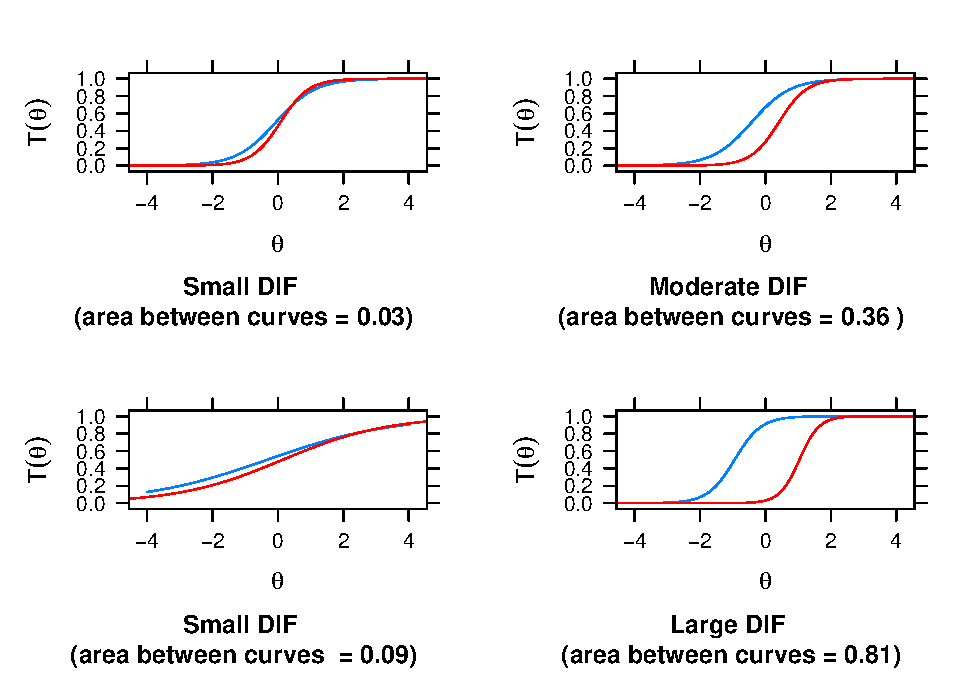
\includegraphics{ICC_project_files/figure-latex/plotting-1.pdf}
\caption{\label{fig:plotting}Four ICCs showcasing the difference between CTT and IRT-derivated curves at different levels.}
\end{figure}

\begin{figure}
\centering
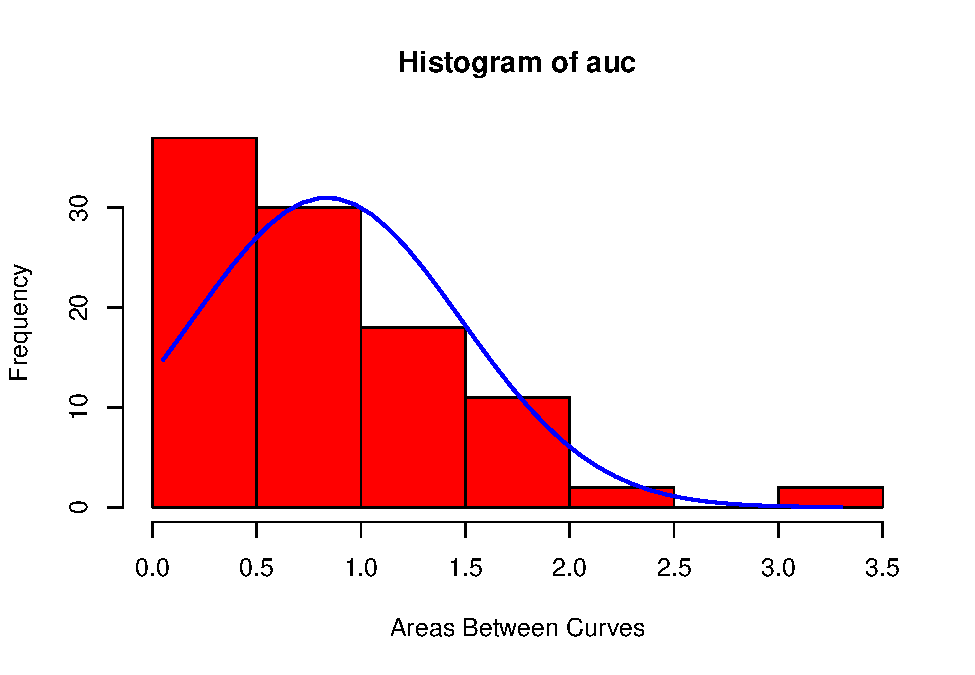
\includegraphics{ICC_project_files/figure-latex/histrogram-1.pdf}
\caption{\label{fig:histrogram}Histogram of all areas between curves plotted using IRT parameters vs curves plotted using CTT parameters.}
\end{figure}

\begin{figure}
\centering
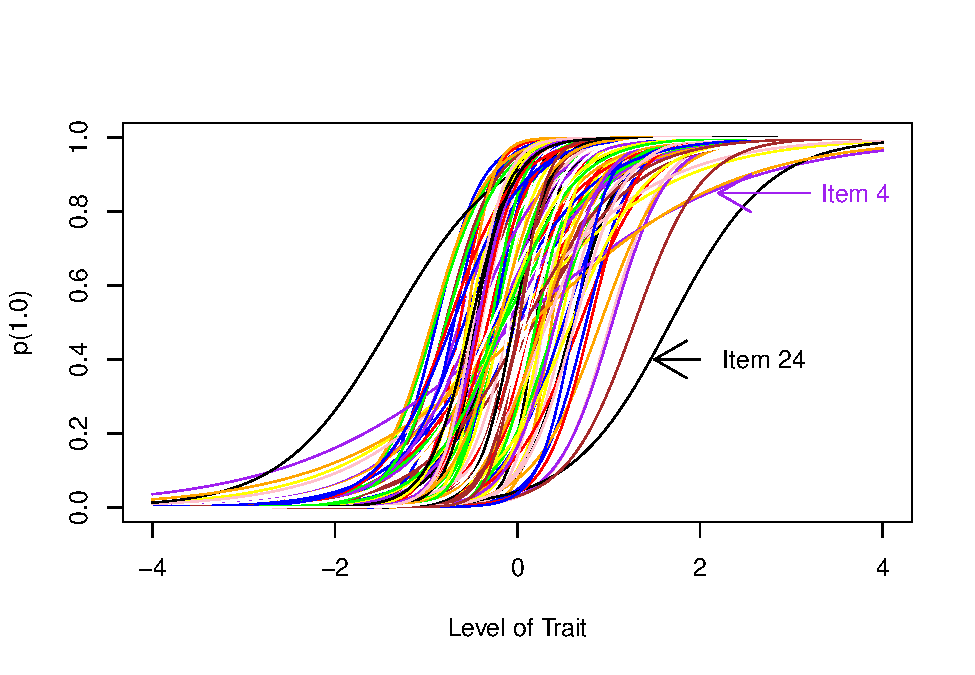
\includegraphics{ICC_project_files/figure-latex/cttcurves-1.pdf}
\caption{\label{fig:cttcurves}ICCs derived from only CTT parameters (with two noteworthy ICCs annotated).}
\end{figure}

\begin{figure}
\centering
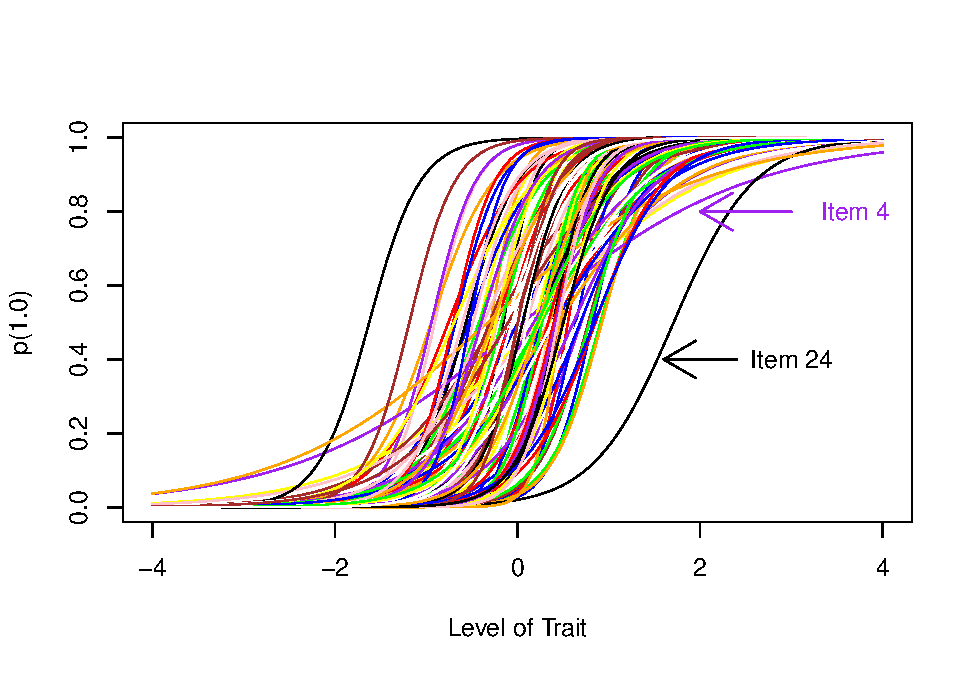
\includegraphics{ICC_project_files/figure-latex/irtcurves-1.pdf}
\caption{\label{fig:irtcurves}Typical ICCs derived from IRT parameters (same noteworthy items annotated).}
\end{figure}

\hypertarget{discussion}{%
\section{Discussion}\label{discussion}}

Important psychometric information can be gathered from ICC's, which are visual indicators typically of difficulty and discrimination. Psychometricians and other assessment specialists usually examine ICC's under the lenses of IRT and Rasch models. From a CTT orientation, item difficulty is most commonly represented by the percent of individuals answering the item correctly (also referred to as a p-value). Item discrimination can be conveyed via a few CTT indices, but the most commonly calculated and consulted index is the corrected item-total correlation. Assessment specialists who consult these CTT parameters don't typically attempt to represent them visually, as is common in IRT and Rasch applications. However, there is perhaps little reason for them not to do so, as ICC's based on CTT parameters could provide snapshot psychometric information as valuable as those gained from IRT- or Rasch-derived ICC's. Here we first propose an application of ICC's with CTT indices, then we simulated data and quantified similarities and discrepancies between the IRT- and CTT-generated ICC's. Our hypothesis was that the Area Between Curves of these different ICC's would be small. Area between curves for 100 items was 0.35 on average. This result indicates that curves plotted with either IRT or CTT parameters show little difference. The nature of both models is mostly overlapping when it comes to plotting visual representations such as ICC's. Practitioners and researchers that don't use IRT or Rasch models and instead opt to follow a CTT philosophy would benefit from having ICC's that use CTT statistics.

If this general idea is well-received (SIOP members would seem to represent a great barometer!) we would like to stress the CTT ICC's via further and more extensive conditions. That is, are there patterns that help explain CTT ICCs that diverge from their IRT counterparts? Although our simulations did generate a range of item difficulties and discriminations, we have not yet fully explored systematic patterns of extremely difficult/easy items as well as very poorly discriminating items. If patterns emerge, we would like to model predicted discrepancies via incorporating error bars within our visualizations.

represent some promise regarding plotted ICC's using IRT and CTT parameters. Our hypothesis was that the Area Between Curves of these different ICCs would be small. Area between curves for 100 items was 0.35 on average. This result indicates that curves plotted with either IRT or CTT parameters show little difference. The nature of both models is overlapping when it comes to plotting visual representations such as ICC's. Practitioners and researchers that don't use IRT or Rasch models and instead opt to follow a CTT philosophy would benefit from having ICC's that use CTT statistics.

Additionally, if there is interest in this general idea we would likely publish our function as a small \texttt{R} package, perhaps to supplement the \texttt{psych} package's ``alpha'' function, which produces corrected item-total correlations as well as p-values within the same output table (e.g., the ``input'' data is already available in tabular format).

\newpage

\hypertarget{references}{%
\section{References}\label{references}}

\begingroup
\setlength{\parindent}{-0.5in}
\setlength{\leftskip}{0.5in}

\hypertarget{refs}{}
\begin{CSLReferences}{1}{0}
\leavevmode\vadjust pre{\hypertarget{ref-R-geiger_a}{}}%
Alfaro, M., Santini, F., Brock, C., Alamillo, H., Dornburg, A., Rabosky, D., Carnevale, G., \& Harmon, L. (2009). Nine exceptional radiations plus high turnover explain species diversity in jawed vertebrates. \emph{Proceedings of the National Academy of Sciences of the United States of America}, \emph{106}, 13410--13414.

\leavevmode\vadjust pre{\hypertarget{ref-R-markdown}{}}%
Allaire, J., Horner, J., Xie, Y., Marti, V., \& Porte, N. (2019). \emph{Markdown: Render markdown with the c library 'sundown'}. \url{https://CRAN.R-project.org/package=markdown}

\leavevmode\vadjust pre{\hypertarget{ref-R-gridExtra}{}}%
Auguie, B. (2017). \emph{gridExtra: Miscellaneous functions for "grid" graphics}. \url{https://CRAN.R-project.org/package=gridExtra}

\leavevmode\vadjust pre{\hypertarget{ref-R-papaja}{}}%
Aust, F., \& Barth, M. (2020). \emph{{papaja}: {Create} {APA} manuscripts with {R Markdown}}. \url{https://github.com/crsh/papaja}

\leavevmode\vadjust pre{\hypertarget{ref-R-tinylabels}{}}%
Barth, M. (2022). \emph{{tinylabels}: Lightweight variable labels}. \url{https://cran.r-project.org/package=tinylabels}

\leavevmode\vadjust pre{\hypertarget{ref-R-mirt}{}}%
Chalmers, R. P. (2012). {mirt}: A multidimensional item response theory package for the {R} environment. \emph{Journal of Statistical Software}, \emph{48}(6), 1--29. \url{https://doi.org/10.18637/jss.v048.i06}

\leavevmode\vadjust pre{\hypertarget{ref-R-descr}{}}%
Dirk Enzmann, J. Aquino. I. R. source code and/or documentation written by, Schwartz, M., Jain, N., \& Kraft, S. (2021). \emph{Descr: Descriptive statistics}. \url{https://CRAN.R-project.org/package=descr}

\leavevmode\vadjust pre{\hypertarget{ref-R-geiger_b}{}}%
Eastman, J., Alfaro, M., Joyce, P., Hipp, A., \& Harmon, L. (2011). A novel comparative method for identifying shifts in the rate of character evolution on trees. \emph{Evolution}, \emph{65}, 3578--3589.

\leavevmode\vadjust pre{\hypertarget{ref-fan1998item}{}}%
Fan, X. (1998). Item response theory and classical test theory: An empirical comparison of their item/person statistics. \emph{Educational and Psychological Measurement}, \emph{58}(3), 357--381.

\leavevmode\vadjust pre{\hypertarget{ref-R-installr}{}}%
Galili, T. (2021). \emph{Installr: Using r to install stuff on windows OS (such as: R, 'rtools', 'RStudio', 'git', and more!)}. \url{https://CRAN.R-project.org/package=installr}

\leavevmode\vadjust pre{\hypertarget{ref-hambleton1993comparison}{}}%
Hambleton, R. K., \& Jones, R. W. (1993). Comparison of classical test theory and item response theory and their applications to test development. \emph{Educational Measurement: Issues and Practice}, \emph{12}(3), 38--47.

\leavevmode\vadjust pre{\hypertarget{ref-hambleton1991fundamentals}{}}%
Hambleton, R. K., Swaminathan, H., \& Rogers, H. J. (1991). \emph{Fundamentals of item response theory} (Vol. 2). Sage.

\leavevmode\vadjust pre{\hypertarget{ref-han2007wingen3}{}}%
Han, K. (2007). WinGen3: Windows software that generates IRT parameters and item responses {[}computer program{]}. \emph{Amherst, MA: Center for Educational Assessment, University of Massachusetts Amherst}.

\leavevmode\vadjust pre{\hypertarget{ref-R-geiger_d}{}}%
Harmon, L., Weir, J., Brock, C., Glor, R., \& Challenger, W. (2008). GEIGER: Investigating evolutionary radiations. \emph{Bioinformatics}, \emph{24}, 129--131.

\leavevmode\vadjust pre{\hypertarget{ref-kulas2017approximate}{}}%
Kulas, J. T., Smith, J. A., \& Xu, H. (2017). Approximate functional relationship between IRT and CTT item discrimination indices: A simulation, validation, and practical extension of lord's (1980) formula. \emph{Journal of Applied Measurement}, \emph{18}(4), 393--407.

\leavevmode\vadjust pre{\hypertarget{ref-R-irtplay}{}}%
Lim, H. (2020). \emph{Irtplay: Unidimensional item response theory modeling}. \url{https://CRAN.R-project.org/package=irtplay}

\leavevmode\vadjust pre{\hypertarget{ref-lord2012applications}{}}%
Lord, F. M. (2012). \emph{Applications of item response theory to practical testing problems}. Routledge.

\leavevmode\vadjust pre{\hypertarget{ref-macdonald2002monte}{}}%
Macdonald, P., \& Paunonen, S. V. (2002). A monte carlo comparison of item and person statistics based on item response theory versus classical test theory. \emph{Educational and Psychological Measurement}, \emph{62}(6), 921--943.

\leavevmode\vadjust pre{\hypertarget{ref-R-geiger_e}{}}%
Pennell, M., Eastman, J., Slater, G., Brown, J., Uyeda, J., Fitzjohn, R., Alfaro, M., \& Harmon, L. (2014). Geiger v2.0: An expanded suite of methods for fitting macroevolutionary models to phylogenetic trees. \emph{Bioinformatics}, \emph{30}, 2216--2218.

\leavevmode\vadjust pre{\hypertarget{ref-R-base}{}}%
R Core Team. (2020). \emph{R: A language and environment for statistical computing}. R Foundation for Statistical Computing. \url{https://www.R-project.org/}

\leavevmode\vadjust pre{\hypertarget{ref-R-psych}{}}%
Revelle, W. (2021). \emph{Psych: Procedures for psychological, psychometric, and personality research}. Northwestern University. \url{https://CRAN.R-project.org/package=psych}

\leavevmode\vadjust pre{\hypertarget{ref-rupp2004note}{}}%
Rupp, A. A., \& Zumbo, B. D. (2004). A note on how to quantify and report whether IRT parameter invariance holds: When pearson correlations are not enough. \emph{Educational and Psychological Measurement}, \emph{64}(4), 588--599.

\leavevmode\vadjust pre{\hypertarget{ref-R-lattice}{}}%
Sarkar, D. (2008). \emph{Lattice: Multivariate data visualization with r}. Springer. \url{http://lmdvr.r-forge.r-project.org}

\leavevmode\vadjust pre{\hypertarget{ref-R-latticeExtra}{}}%
Sarkar, D., \& Andrews, F. (2019). \emph{latticeExtra: Extra graphical utilities based on lattice}. \url{https://CRAN.R-project.org/package=latticeExtra}

\leavevmode\vadjust pre{\hypertarget{ref-R-geiger_c}{}}%
Slater, G., Harmon, L., Wegmann, D., Joyce, P., Revell, L., \& Alfaro, M. (2012). Fitting models of continuous trait evolution to incompletely sampled comparative data using approximate bayesian computation. \emph{Evolution}, \emph{66}, 752--762.

\leavevmode\vadjust pre{\hypertarget{ref-R-reticulate}{}}%
Ushey, K., Allaire, J., \& Tang, Y. (2021). \emph{Reticulate: Interface to 'python'}. \url{https://CRAN.R-project.org/package=reticulate}

\leavevmode\vadjust pre{\hypertarget{ref-R-ggplot2}{}}%
Wickham, H. (2016). \emph{ggplot2: Elegant graphics for data analysis}. Springer-Verlag New York. \url{https://ggplot2.tidyverse.org}

\leavevmode\vadjust pre{\hypertarget{ref-R-usethis}{}}%
Wickham, H., Bryan, J., \& Barrett, M. (2021). \emph{Usethis: Automate package and project setup}. \url{https://CRAN.R-project.org/package=usethis}

\leavevmode\vadjust pre{\hypertarget{ref-R-devtools}{}}%
Wickham, H., Hester, J., Chang, W., \& Bryan, J. (2021). \emph{Devtools: Tools to make developing r packages easier}. \url{https://CRAN.R-project.org/package=devtools}

\leavevmode\vadjust pre{\hypertarget{ref-R-knitr}{}}%
Xie, Y. (2015). \emph{Dynamic documents with {R} and knitr} (2nd ed.). Chapman; Hall/CRC. \url{https://yihui.org/knitr/}

\leavevmode\vadjust pre{\hypertarget{ref-R-tinytex}{}}%
Xie, Y. (2019). TinyTeX: A lightweight, cross-platform, and easy-to-maintain LaTeX distribution based on TeX live. \emph{TUGboat}, \emph{1}, 30--32. \url{http://tug.org/TUGboat/Contents/contents40-1.html}

\leavevmode\vadjust pre{\hypertarget{ref-R-rmarkdown_a}{}}%
Xie, Y., Allaire, J. J., \& Grolemund, G. (2018). \emph{R markdown: The definitive guide}. Chapman; Hall/CRC. \url{https://bookdown.org/yihui/rmarkdown}

\leavevmode\vadjust pre{\hypertarget{ref-R-rmarkdown_b}{}}%
Xie, Y., Dervieux, C., \& Riederer, E. (2020). \emph{R markdown cookbook}. Chapman; Hall/CRC. \url{https://bookdown.org/yihui/rmarkdown-cookbook}

\end{CSLReferences}

\endgroup


\end{document}
